The inference part contains the 4 following functionalities:

\begin{itemize}
\item \mintinline{python}{romc.sample(n2, seed=None)}
\item \mintinline{python}{romc.eval_unnorm_posterior(theta)}
\item \mintinline{python}{romc.eval_posterior(theta)}
\item \mintinline{python}{romc.compute_expectation(h)}
\end{itemize}

\subsubsection*{Function (i): \mintinline{python}{romc.sample(n2)}}

This is the basic inference utility of the ROMC implementation. The
samples are drawn from a uniform distribution $q_i$ defined over the
corresponding bounding box and the weight $w_i$ is computed as in
equation~\eqref{eq:sampling}. The function stores an
\pinline{elfi.Result} object as \pinline{romc.result} attribute. The
\pinline{elfi.Result} provides by some usefull functionalities for
inspecting the obtained samples such as
\pinline{romc.result.summary()} that prints the number. A comlete
overview of these functionalities is provided in ELFI's
\href{https://elfi.readthedocs.io/en/latest/api.html#elfi.methods.results.Sample}{official
  documentation}.

\subsubsection*{Function (ii):nn
  \mintinline{python}{romc.compute_expectation(h)}}

This function computes the expectation
$E_{p(\thetab|\data)}[h(\thetab)]$ using the
expression~\eqref{eq:expectation}. The argument \pinline{h} can be
any python \pinline{Callable} that accepts a one-dimensional
\pinline{np.ndarray} as input and returns a one-dimensional
\pinline{np.ndarray} as output.

\subsubsection*{Function (iii):
  \mintinline{python}{romc.eval_unorm_posterior(theta)}}

This function computes the unnormalised posterior approximation using
the expression~\eqref{eq:approx_posterior}.

\subsubsection*{Function (iv):
  \mintinline{python}{romc.eval_posterior(theta)}}

This function evaluates the normalised posterior. For doing so it
needs to approximate the partition function
$Z = \int_{\thetab : p(\thetab)>0}
p_{d,\epsilon}(\thetab|\data)d\thetab$; this is done using the Riemann
integral aproximation. Unfortunatelly, the Riemann approximation does
not scale well in high-dimensional spaces, hence the approximation is
tractable only at low-dimensional parametric spaces. Given that this
functionality is particulary useful for ploting the posterior, we
could say that it is meaningful to be used for up to $3D$ parametric
spaces, even though it is not restricted to that. Finally, for this
functionality to work, the left and right limit determinining a
bounding box that includes the area where the prior distribution has
mass must have been passed as the \pinline{left_lim, right_lim} in the
initialisation of the \pinline{elfi.ROMC} object.

\subsubsection*{Example - Sampling and compute expectation}

With the following code snippet, we perform weighted sampling from the
ROMC approximate posterior. Afterwards, we used some ELFI's built-in
tools to get a summary of the obtained samples. In figure
\ref{fig:example_sampling}, we observe the histogram of the weighted
samples and the acceptance region of the first deterministic function
(as before) alongside with the obtained samples obtained from
it. Finally, in the code snippet we demonstrate how to use the
\pinline{compute_expectation} function; in the current example we
define \pinline{h} in order to compute firstly the empirical mean and
afterwards the empirical variance. In both cases, the empirical result
is close to the ground truth $\mu = 0$ and $\sigma^2 = 1$.

\begin{pythoncode}
  seed = 21
  n2 = 50
  romc.sample(n2=n2, seed=seed)

  # visualize region, adding the samples now
  romc.visualize_region(i=1)

  # Visualise marginal (built-in ELFI tool)
  romc.result.plot_marginals(weights=romc.result.weights, bins=100, range=(-3,3))

  # Summarize the samples (built-in ELFI tool)
  romc.result.summary()
  # Number of samples: 1720
  # Sample means: theta: -0.0792

  # compute expectation
  print("Expected value   : %.3f" % romc.compute_expectation(h=lambda x: np.squeeze(x)))
  # Expected value   : -0.079

  print("Expected variance: %.3f" % romc.compute_expectation(h=lambda x: np.squeeze(x)**2))
  # Expected variance: 1.061
\end{pythoncode}

\begin{figure}[h]
    \begin{center}
      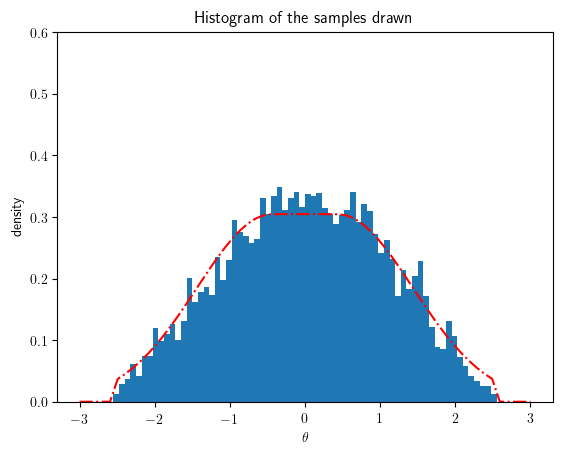
\includegraphics[width=0.48\textwidth]{./Thesis/images/chapter3/example_marginal.png}
      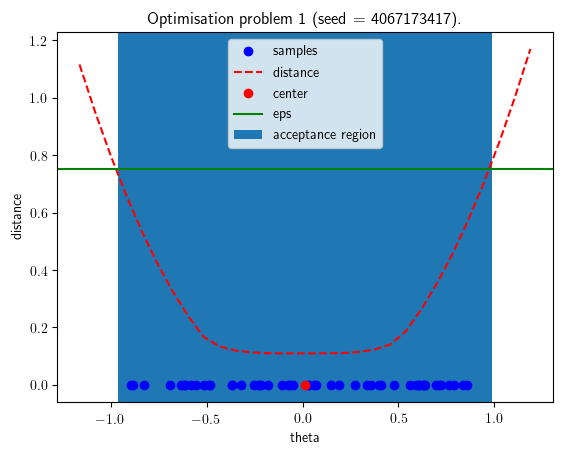
\includegraphics[width=0.48\textwidth]{./Thesis/images/chapter3/example_region_samples.png}
    \end{center}
  \caption{(a) Left: Histogram of the obtained samples. (b) Right: Acceptance region around $\theta_1^*$ with the obtained samples ploted inside.}
  \label{fig:example_sampling}
\end{figure}

\subsubsection*{Example - Evaluate Posterior}

The \pinline{romc.eval_unnorm_posterior(theta)} evaluates the
posterior at point $\theta$ using the expression
\eqref{eq:aprox_posterior}. The \pinline{romc.eval_posterior(theta)}
approximates the partition function
$Z = \int_{\thetab} p_{d,\epsilon}(\thetab|\data) d\thetab$ using the
Riemann approximation in the points where the prior has mass; hence it
doesn't scale well to high-dimensional spaces. In our simple example,
this utility can provide a nice plot of the approximate posterior as
illustrated in figure~\ref{fig:approx_posterior}. We observe that the
approximation is quite close to the ground-truth posterior.

\begin{figure}[h]
    \begin{center}
      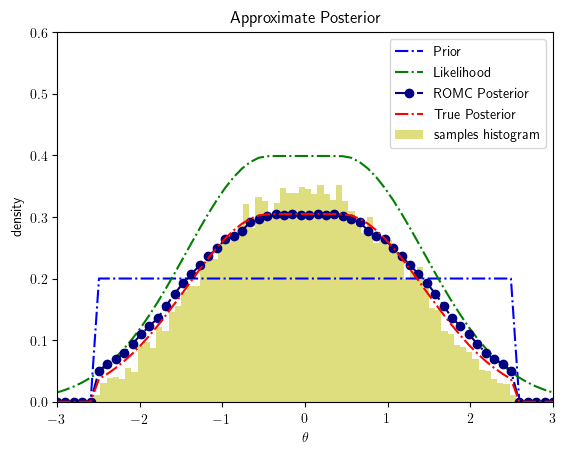
\includegraphics[width=0.75\textwidth]{./Thesis/images/chapter3/example_posterior.png}
    \end{center}
  \caption{Approximate posterior evaluation.}
  \label{fig:approx_posterior}
\end{figure}
